\documentclass[10pt,a4paper]{article}
\usepackage[utf8]{inputenc}
\usepackage{amsmath}
\usepackage{amsfonts}
\usepackage{amssymb}
\usepackage{siunitx}
\usepackage{graphicx}
\usepackage{subfig}
\usepackage{hyperref}
\begin{document}
\title{Assignment I - Bhabha scattering}
\author{Federico Nardi}
\maketitle
The solution to the first two problems is presented in the attached sheets at the end of the paper. The $\gamma$ matrices properites used are from \cite{mysaviour}.\\

The code used for this project can be found here:\\
\url{https://github.com/FedericoNardi/ParticlePhysics.git}
\section{Differential Cross Section}
Starting from the expression for the matrix element
\begin{align*}
<|M_{fi}|^2> = 4e^4\bigg[& 2\frac{(p_1 \cdot p_4)(p_2 \cdot p_3)+(p_1 \cdot p_3)(p_2 \cdot p_4)}{s^2}
+
2\frac{(p_3 \cdot p_4)(p_1 \cdot p_2)+(p_1 \cdot p_4)(p_3 \cdot p_2)}{t^2}+\\
-
&\frac{(p_1 \cdot p_4)(p_3 \cdot p_2)}{st}
 \bigg]\\ 
&\text{where}\quad s=(p_1+p_2)^2=(p_3+p_4)^2\quad \text{and}\quad t=(p_1-p_3)^2=(p_2-p_4)^2
\end{align*} 
and inserting the expressions for momenta in the \textbf{center-mass frame}
\begin{align*}
&p_1 = (E,0,0,E)\\
&p_2 = (E,0,0,-E)\\
&p_3 = (E,0,E\sin\theta,E\cos\theta)\\
&p_4 = (E,0,-E\sin\theta,-E\cos\theta)
\end{align*}
we get the identities 
\begin{align*}
&p_2 \cdot p_3 = E^2(1-\cos\theta) = p_1 \cdot p_4\\
&p_1 \cdot p_3 = E^2(1-\cos\theta) = p_2 \cdot p_4\\
&p_3 \cdot p_4 = 2E^2 = p_1 \cdot p_2\\
&s = 4E^2\\
&t = 2E^2(1-\cos\theta)
\end{align*}
and therefore the expression for the matrix element, with $e^2=4\pi\alpha$ becomes
\begin{align*}
<|M_{fi}|^2> = (4\pi\alpha)^2\bigg[ \underbrace{\frac{(1+\cos\theta)^2+(1-\cos\theta)^2}{2}}_{\text{Annihilation contribution}} + \underbrace{\frac{8+2(1+\cos\theta)^2}{(1-\cos\theta)^2}}_{\text{scattering contribution}} - \underbrace{\frac{(1+\cos\theta)^2}{1-\cos\theta}}_{\text{cross term contr.}}\bigg].
\end{align*}
The expression for the Lorentz-invariant differential cross section is
\begin{align*}
\frac{d\sigma}{dt} = \frac{1}{64\pi\,s|\vec{p_1}|^2}<|M_{fi}|^2>
\end{align*}
we can get an expression for our reference system by substituting the differential
$dt = 2|\vec{p}_1|\,|\vec{p}_3|d(\cos\theta)$:
\begin{align}
\label{eq:diffcross}
\frac{d\sigma}{d(\cos\theta)} = \frac{1}{32\pi\,s}<|M_{fi}|^2>
\end{align}
since in our frame $|\vec{p}_1|=|\vec{p}_3|=E$.\\

Using the values $E = \frac{\sqrt{s}}{2} = 7\si{\giga\electronvolt}$, $e^2=4\pi\alpha = \frac{4\pi}{137}$, equation \ref{eq:diffcross} has been implemented on a Python code evaluating it for various values of $\cos\theta$. Figure \ref{fig:crossection} shows the differential cross section from equation \ref{eq:diffcross} evaluated at different angles, while in figure \ref{fig:CScontribs} each component of the total matrix element contribution is isolated.

\begin{figure}[!ht]
\centering
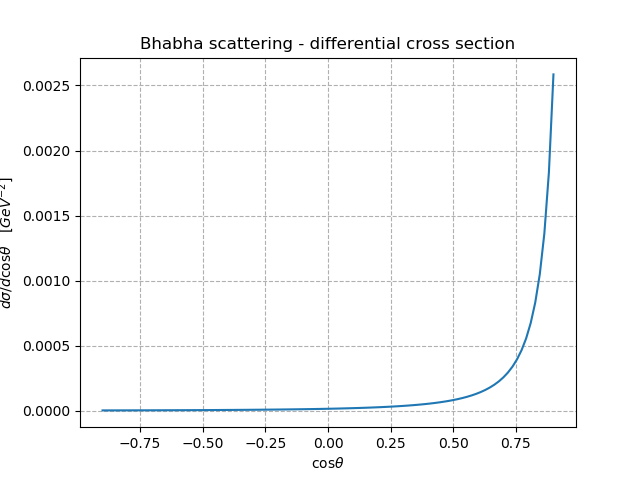
\includegraphics[width=0.7\textwidth]{figures/differentialCS.png}
\caption{Angular dependence of differential cross section for electron-positron scattering}
\label{fig:crossection}
\end{figure}

\begin{figure}[!ht]
\centerline{
\subfloat[s-channel]{
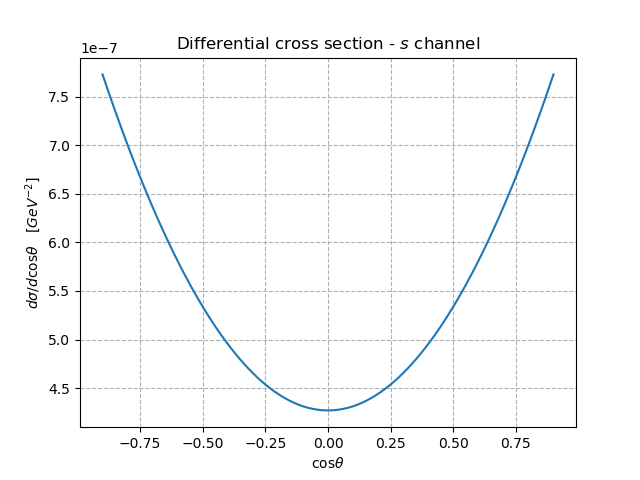
\includegraphics[width=0.45\textwidth]{figures/annihilationCS}
}
\subfloat[t-channel]{
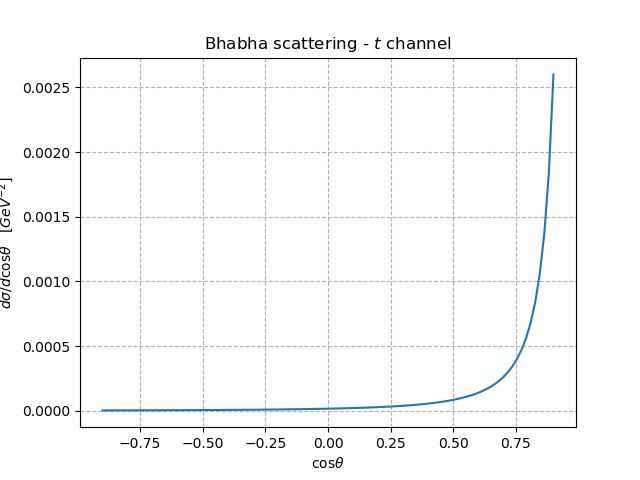
\includegraphics[width=0.45\textwidth]{figures/scatteringCS}
}
\subfloat[cross term]{
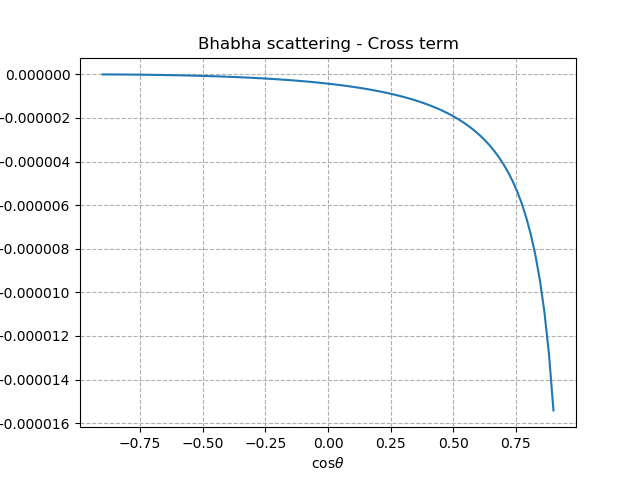
\includegraphics[width=0.45\textwidth]{figures/crossCS}
}
}
\caption{Different contribution for the differential cross section.}
\label{fig:CScontribs}
\end{figure}

It is clear that the dominant contribution to the differential cross section for the process comes from the t-channel (scattering), while the interference cross term has a soft damping effect only for small angles $\cos\theta\sim1$.

Using the result derived in the lectures for $e^+e^-\rightarrow\mu^+\mu^-$
\begin{align*}
\frac{d\sigma}{d(\cos\theta)} = 2\pi\frac{d\sigma}{d\Omega} = \frac{(4\pi\alpha^2)}{64\pi\,s}\bigg[ (1+cos^2\theta) + (1-\cos^2\theta) \bigg]
\end{align*}
we can note that it is the same expression obtained by combining equation \ref{eq:diffcross} with the first term of the matrix element $<|M_{fi}|^2>$. As expected, in the ultrarelativistic limit $m_{e^{\pm}}\sim m_{\mu^{\pm}} << E$ the masses of the leptons can be neglected and the s-channel processes themselves can produce muons-antimuons and electrons-antielectrons with the same yield.

\section{Total Bhabha Cross Section}
The total cross section for the process is obtained as
\begin{align*}
\sigma = \int_{-1}^1 d(\cos\theta) \frac{d\sigma}{d(\cos\theta)}.
\end{align*}
Since the integral diverges for $cos\theta \rightarrow 1$, a cut-off $\epsilon$ has been introduced in the integration domain that becomes $[-1,1-\epsilon]$. The integral has been evaluated numerically for $\epsilon=0.001$ and for different values of center mass energies, and the results are shown in figure \ref{fig:totalcrossection}.

\begin{figure}[!ht]
\centering
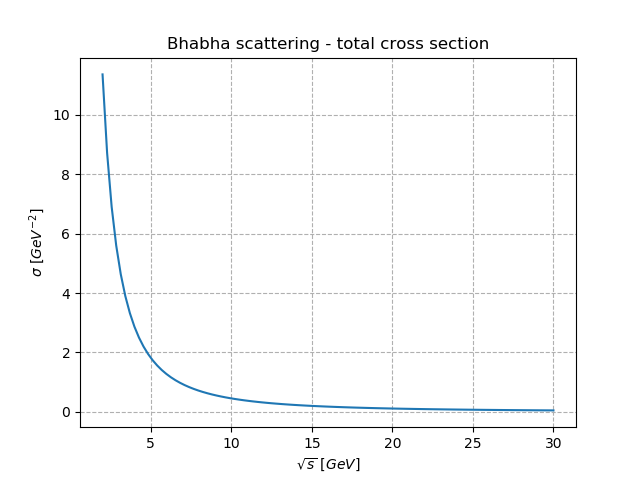
\includegraphics[width=0.7\textwidth]{figures/totalCS.png}
\caption{Energy dependence of total cross section for electron-positron scattering}
\label{fig:totalcrossection}
\end{figure}

The behaviour of the total cross section is as expected $\propto E^{-2}$, since the only energy dependence is in the prefactor of equation \ref{eq:diffcross}, that goes as $1/s$.\\
Due to the fact that the differential cross section diverges for small angles, the result is strongly dependent on the chosen cut off, i.e. the effective (small) scattering angles that an hypothetical detector is sensitive to.\\

For $\sqrt{s}=14\si{\giga\electronvolt}$ the total cross section is
\begin{align*}
\sigma  = 0.232\,\si{\per\square\giga\electronvolt} = 90.3\,\si{\micro\barn}
\end{align*}
being $1\si{\per\square\giga\electronvolt}=0.3894\,\si{\pico\barn}$.
For a beam with integrated luminosity $\mathcal{L}=10\,\si{\per\pico\barn}$ and a $50\si{\percent}$ acceptance efficiency, the expected number of events detected is
\begin{align*}
N = \sigma\,\mathcal{L}\,\times \text{efficiency} = 4.5\times10^8\,\text{events}
\end{align*}
assuming that our setup detects events up to very small scattering angles.\\

The total cross section for the muon pair production process $e^+e^-\rightarrow\mu^+\mu^-$ is shown in figure \ref{fig:muontotalcrossection}. The behaviour is the same as for Bhabha scattering for the same argument as before, however for this process the total cross section is much smaller: the differential cross section does not diverge for any angle (see figure \ref{fig:CScontribs}a) and there was no need to introduce a cut-off in the integral. This implies a much smaller contribution to the total cross section for small angles.

\begin{figure}[!ht]
\centering
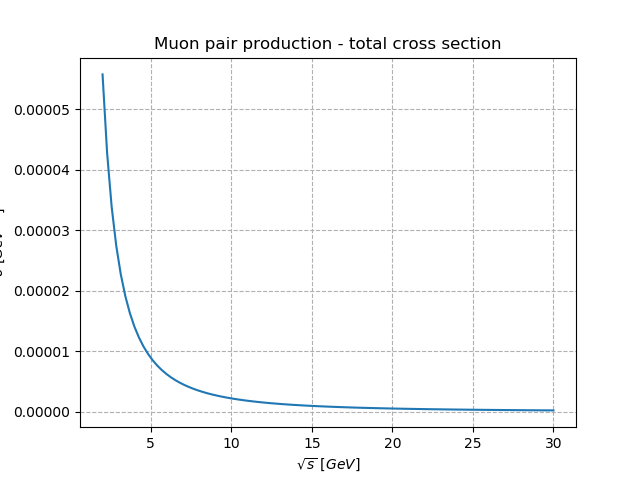
\includegraphics[width=0.7\textwidth]{figures/muontotalCS.png}
\caption{Energy dependence of total cross section for electron-positron scattering}
\label{fig:muontotalcrossection}
\end{figure}

In fact, for this process the total cross section at $\sqrt{s}=14\si{\giga\electronvolt}$ is
\begin{align*}
\sigma  = 1.14\times10^{-6}\,\si{\per\square\giga\electronvolt} = 443\,\si{\pico\barn}
\end{align*}

\section{Comparison with experimental results}
A comparison with the number of events for Bhabha scattering and muon pair production has been made from \cite{29GeV}.\\
In the article is considered a center mass energy of $29\,\si{\giga\electronvolt}$ with integrated luminosity $\mathcal{L}=19.6\si{\per\pico\barn}$ with angular acceptance $|\cos\theta|<0.55$ and $0.75<|\cos\theta|<0.85$. With a $99\si{\percent}$ events sensitivity and a $12\si{\percent}$ dead time, a $88\si{\percent}$ acceptance sensitivity has been considered.
The expected number of events is therefore:
\begin{align*}
10^5\,\text{events}\qquad \text{for	}e^+e^-\rightarrow e^+e^-\\
200\,\text{events}\qquad \text{for	}e^+e^-\rightarrow \mu^+\mu^-\\
\end{align*} 
The sample in the article consists in $8915$ $e^+e^-$ events and $811$ $\mu^+\mu^-$ events. While the first one can be compatible with our estimation, the latter is 4 times higher. This may be due to a too shallow analysis of the detector system from my part.

\begin{thebibliography}{2}

\bibitem{mysaviour}
\url{http://bolvan.ph.utexas.edu/~vadim/	classes/2008f.homeworks/traceology.pdf}

\bibitem{29GeV}
	D. Bender et al., \textit{Tests of QED at 29 GeV center-of-mass energy}, Phys. Rev. D 30, 515 – Published 1 August 1984
	
\end{thebibliography}
 
\end{document}